\documentclass[conference]{IEEEtran}
\usepackage{times}

% numbers option provides compact numerical references in the text.
\usepackage[numbers]{natbib}
\usepackage{multicol}
\usepackage[bookmarks=true]{hyperref}

\usepackage{graphicx} % more modern
%\usepackage{epsfig} % less modern
\usepackage{subfigure}

% For algorithms
\usepackage{algorithm}
\usepackage{algorithmic}
\usepackage{amsmath}
\usepackage{amssymb}
% Include other packages here, before hyperref.
\usepackage{color}
\usepackage{setspace}
\usepackage{wrapfig}
\usepackage{dsfont}

\usepackage[it,small]{caption}


\newcommand{\argmax}{\operatorname{arg\,max}}
\newcommand{\argmin}{\operatorname{arg\,min}}
\newcommand{\todo}[1]{\textcolor{blue}{\textbf{#1}}}
\newtheorem{mydef}{Definition}



\graphicspath{{./images/}}
\usepackage{multirow}
% Some illegal space-saving macros
% \parskip=1pt
  \abovedisplayskip 3.0pt plus2pt minus2pt%
 \belowdisplayskip \abovedisplayskip
\renewcommand{\baselinestretch}{0.97}

\newenvironment{packed_enum}{
\begin{enumerate}
  \setlength{\itemsep}{0pt}
  \setlength{\parskip}{0pt}
  \setlength{\parsep}{0pt}
}
{\end{enumerate}}

\newenvironment{packed_item}{
\begin{itemize}
  \setlength{\itemsep}{0pt}
  \setlength{\parskip}{0pt}
  \setlength{\parsep}{0pt}
}{\end{itemize}}

\newlength\savedwidth
\newcommand\whline[1]{\noalign{\global\savedwidth\arrayrulewidth
                               \global\arrayrulewidth #1} %
                      \hline
                      \noalign{\global\arrayrulewidth\savedwidth}}

% \renewcommand\multirowsetup{\centering}

\newlength{\sectionReduceTop}
\newlength{\sectionReduceBot}
\newlength{\subsectionReduceTop}
\newlength{\subsectionReduceBot}
\newlength{\abstractReduceTop}
\newlength{\abstractReduceBot}
\newlength{\captionReduceTop}
\newlength{\captionReduceBot}
%\newlength{\nameReduceTop}
\newlength{\subsubsectionReduceTop}
\newlength{\subsubsectionReduceBot}
\newlength{\headerReduceTop}
% Negative space for figures set at the bottom of a block of figs
\newlength{\figureReduceBot}

\newlength{\horSkip}
\newlength{\verSkip}

\newlength{\equationReduceTop}

\newlength{\figureHeight}
\setlength{\figureHeight}{1.7in}

%\newlength{\figureFraction}
\setlength{\horSkip}{-.09in}
\setlength{\verSkip}{-.1in}
%\setlength{\figureFraction}{.195}

% figureReduceBot is for figures which are set above text, since latex
% likes putting a lot of space under those
\setlength{\figureReduceBot}{-0.15in}
\setlength{\headerReduceTop}{0in}
%
%\setlength{\subsectionReduceTop}{-0.08in}
%\setlength{\subsectionReduceBot}{-0.05in}
\setlength{\subsectionReduceTop}{-0.02in}
\setlength{\subsectionReduceBot}{-0.02in}
%\setlength{\sectionReduceTop}{-0.03in}
%\setlength{\sectionReduceBot}{-0.03in}
\setlength{\sectionReduceTop}{-0.02in}
\setlength{\sectionReduceBot}{-0.01in}
\setlength{\subsubsectionReduceTop}{-0.06in}
\setlength{\subsubsectionReduceBot}{-0.05in}
%
%
%\setlength{\figureHeight}{1.5in}
\setlength{\abstractReduceTop}{-0.05in}
\setlength{\abstractReduceBot}{-0.10in}
%
%

\setlength{\equationReduceTop}{-0.1in}

%\setlength{\nameReduceTop}{-0.05in}


\setlength{\captionReduceTop}{-0.06in}
\setlength{\captionReduceBot}{-0.07in}



\pdfinfo{
   /Author (Homer Simpson)
   /Title  (Robots: Our new overlords)
   /CreationDate (D:20101201120000)
   /Subject (Robots)
   /Keywords (Robots;Overlords)
}

\usepackage{helvet}
%\renewcommand{\familydefault}{\sfdefault}

\begin{document}


% paper title
\title{Supplementary Material For \\ rCRF: Recursive Belief Estimation over CRFs in RGB-D Activity Videos}

% You will get a Paper-ID when submitting a pdf file to the conference system
%\author{Author Names Omitted for Anonymous Review. Paper-ID 63}
\author{
\authorblockN{Ozan Sener}
\authorblockA{School of Electrical \& Computer Eng. \\ Cornell University}
\and
\authorblockN{Ashutosh Saxena}
\authorblockA{Department of Computer Science \\ Cornell University}
}


\maketitle

\IEEEpeerreviewmaketitle
\section{Qualitative Results}
\begin{figure}[ht]
\small
%\begin{singlespace}
\begin{tabular}{p{5mm}@{}l}
\begin{tabular}{r}
\rotatebox[origin=r]{90}{\;\;\;\;\;\;\;Middle Frame}\\
\rotatebox[origin=l]{90}{Belief\;\;\;\;\;\;\;}
\end{tabular}
&
\begin{tabular}{p{3.7cm}p{3.7cm}p{3.7cm}p{3.7cm}}
\includegraphics[width=0.225\textwidth]{f10} &
\includegraphics[width=0.225\textwidth]{f11} &
\includegraphics[width=0.225\textwidth]{f12} &
\includegraphics[width=0.225\textwidth]{f13}  \\ %\\%\begin{tabular}{p{3.6cm}p{3.6cm}p{3.6cm}p{3.6cm}}
\includegraphics[width=0.225\textwidth, height=8mm]{P10} &
\includegraphics[width=0.225\textwidth, height=8mm]{P12P} &
\includegraphics[width=0.225\textwidth, height=8mm]{P13P} &
\includegraphics[width=0.225\textwidth, height=8mm]{P14P}  \\

\vspace{-6mm}\hspace{-1mm}\scalebox{0.84}{
\rotatebox[origin=r]{90}{reaching}\hspace{1mm}
\rotatebox[origin=r]{90}{moving}\hspace{1mm}
\rotatebox[origin=r]{90}{pouring}\hspace{1mm}
\rotatebox[origin=r]{90}{eating}\hspace{1mm}
\rotatebox[origin=r]{90}{drinking}\hspace{1mm}
\rotatebox[origin=r]{90}{opening}\hspace{1mm}
\rotatebox[origin=r]{90}{placing}\hspace{1mm}
\rotatebox[origin=r]{90}{closing}\hspace{1mm}
\rotatebox[origin=r]{90}{null}\hspace{1mm}
\rotatebox[origin=r]{90}{cleaning}}&
\vspace{-6mm}\hspace{-1mm}\scalebox{0.84}{
\rotatebox[origin=r]{90}{reaching}\hspace{1mm}
\rotatebox[origin=r]{90}{moving}\hspace{1mm}
\rotatebox[origin=r]{90}{pouring}\hspace{1mm}
\rotatebox[origin=r]{90}{eating}\hspace{1mm}
\rotatebox[origin=r]{90}{drinking}\hspace{1mm}
\rotatebox[origin=r]{90}{opening}\hspace{1mm}
\rotatebox[origin=r]{90}{placing}\hspace{1mm}
\rotatebox[origin=r]{90}{closing}\hspace{1mm}
\rotatebox[origin=r]{90}{null}\hspace{1mm}
\rotatebox[origin=r]{90}{cleaning}}&
\vspace{-6mm}\hspace{-1mm}\scalebox{0.84}{
\rotatebox[origin=r]{90}{reaching}\hspace{1mm}
\rotatebox[origin=r]{90}{moving}\hspace{1mm}
\rotatebox[origin=r]{90}{pouring}\hspace{1mm}
\rotatebox[origin=r]{90}{eating}\hspace{1mm}
\rotatebox[origin=r]{90}{drinking}\hspace{1mm}
\rotatebox[origin=r]{90}{opening}\hspace{1mm}
\rotatebox[origin=r]{90}{placing}\hspace{1mm}
\rotatebox[origin=r]{90}{closing}\hspace{1mm}
\rotatebox[origin=r]{90}{null}\hspace{1mm}
\rotatebox[origin=r]{90}{cleaning}}&
\vspace{-6mm}\hspace{-1mm}\scalebox{0.84}{
\rotatebox[origin=r]{90}{reaching}\hspace{1mm}
\rotatebox[origin=r]{90}{moving}\hspace{1mm}
\rotatebox[origin=r]{90}{pouring}\hspace{1mm}
\rotatebox[origin=r]{90}{eating}\hspace{1mm}
\rotatebox[origin=r]{90}{drinking}\hspace{1mm}
\rotatebox[origin=r]{90}{opening}\hspace{1mm}
\rotatebox[origin=r]{90}{placing}\hspace{1mm}
\rotatebox[origin=r]{90}{closing}\hspace{1mm}
\rotatebox[origin=r]{90}{null}\hspace{1mm}
\rotatebox[origin=r]{90}{cleaning}}
\end{tabular}
\end{tabular}

\begin{tabular}{p{5mm}@{}l}
\begin{tabular}{r}
\rotatebox[origin=r]{90}{\;\;\;\;\;\;\;Middle Frame}\\
\rotatebox[origin=l]{90}{Belief\;\;\;\;\;\;\;}
\end{tabular}
&
\begin{tabular}{p{3.7cm}p{3.7cm}p{3.7cm}p{3.7cm}}
\includegraphics[width=0.225\textwidth]{l5} &
\includegraphics[width=0.225\textwidth]{l6} &
\includegraphics[width=0.225\textwidth]{l7} &
\includegraphics[width=0.225\textwidth]{l8}  \\
\includegraphics[width=0.225\textwidth, height=9mm]{bl5} &
\includegraphics[width=0.225\textwidth, height=9mm]{bl6_2} &
\includegraphics[width=0.225\textwidth, height=9mm]{bl7_2} &
\includegraphics[width=0.225\textwidth, height=9mm]{bl8_2}  \\
\iffalse
\begin{tikzpicture}[remember picture,overlay]
\node[anchor=south west,inner sep=0] (image1)
  {\includegraphics[width=0.22\textwidth, height=10mm]{bl5}};
\end{tikzpicture} &
\begin{tikzpicture}[remember picture,overlay]
\node[anchor=south west,inner sep=0] (image2)
  {\includegraphics[width=0.22\textwidth, height=10mm]{bl6_2}};
\end{tikzpicture} &
\begin{tikzpicture}[remember picture,overlay]
\node[anchor=south west,inner sep=0] (image3)
  {\includegraphics[width=0.22\textwidth, height=10mm]{bl7_2}};
\end{tikzpicture} &
\begin{tikzpicture}[remember picture,overlay]
\node[anchor=south west,inner sep=0] (image4)
  {\includegraphics[width=0.22\textwidth, height=10mm]{bl8_2}};
\end{tikzpicture}
\begin{tikzpicture}[remember picture,overlay]
\draw[->,line width=2pt,red!80!black]
([yshift=-5pt,xshift=14pt]image4.west) |-
([yshift=-5pt,xshift=81pt]image3.west);
\draw[->,line width=2pt,red!80!black]
([yshift=0pt,xshift=81pt]image3.west) |-
([yshift=0pt,xshift=13pt]image2.west);
\draw[->,line width=2pt,red!80!black]
([yshift=-5pt,xshift=13pt]image2.west) |-
([yshift=-5pt,xshift=5pt]image1.west);
\end{tikzpicture}
\fi
\vspace{-6mm}\hspace{-1mm}\scalebox{0.84}{
\rotatebox[origin=r]{90}{reaching}\hspace{1mm}
\rotatebox[origin=r]{90}{moving}\hspace{1mm}
\rotatebox[origin=r]{90}{pouring}\hspace{1mm}
\rotatebox[origin=r]{90}{eating}\hspace{1mm}
\rotatebox[origin=r]{90}{drinking}\hspace{1mm}
\rotatebox[origin=r]{90}{opening}\hspace{1mm}
\rotatebox[origin=r]{90}{placing}\hspace{1mm}
\rotatebox[origin=r]{90}{closing}\hspace{1mm}
\rotatebox[origin=r]{90}{null}\hspace{1mm}
\rotatebox[origin=r]{90}{cleaning}}&
\vspace{-6mm}\hspace{-1mm}\scalebox{0.84}{
\rotatebox[origin=r]{90}{reaching}\hspace{1mm}
\rotatebox[origin=r]{90}{moving}\hspace{1mm}
\rotatebox[origin=r]{90}{pouring}\hspace{1mm}
\rotatebox[origin=r]{90}{eating}\hspace{1mm}
\rotatebox[origin=r]{90}{drinking}\hspace{1mm}
\rotatebox[origin=r]{90}{opening}\hspace{1mm}
\rotatebox[origin=r]{90}{placing}\hspace{1mm}
\rotatebox[origin=r]{90}{closing}\hspace{1mm}
\rotatebox[origin=r]{90}{null}\hspace{1mm}
\rotatebox[origin=r]{90}{cleaning}}&
\vspace{-6mm}\hspace{-1mm}\scalebox{0.84}{
\rotatebox[origin=r]{90}{reaching}\hspace{1mm}
\rotatebox[origin=r]{90}{moving}\hspace{1mm}
\rotatebox[origin=r]{90}{pouring}\hspace{1mm}
\rotatebox[origin=r]{90}{eating}\hspace{1mm}
\rotatebox[origin=r]{90}{drinking}\hspace{1mm}
\rotatebox[origin=r]{90}{opening}\hspace{1mm}
\rotatebox[origin=r]{90}{placing}\hspace{1mm}
\rotatebox[origin=r]{90}{closing}\hspace{1mm}
\rotatebox[origin=r]{90}{null}\hspace{1mm}
\rotatebox[origin=r]{90}{cleaning}}&
\vspace{-6mm}\hspace{-1mm}\scalebox{0.84}{
\rotatebox[origin=r]{90}{reaching}\hspace{1mm}
\rotatebox[origin=r]{90}{moving}\hspace{1mm}
\rotatebox[origin=r]{90}{pouring}\hspace{1mm}
\rotatebox[origin=r]{90}{eating}\hspace{1mm}
\rotatebox[origin=r]{90}{drinking}\hspace{1mm}
\rotatebox[origin=r]{90}{opening}\hspace{1mm}
\rotatebox[origin=r]{90}{placing}\hspace{1mm}
\rotatebox[origin=r]{90}{closing}\hspace{1mm}
\rotatebox[origin=r]{90}{null}\hspace{1mm}
\rotatebox[origin=r]{90}{cleaning}}
\end{tabular}
\end{tabular}
\caption{\textbf{Anticipated belief over activity.} In the first and third row, we show a middle frame of the temporal segment. In the second and fourth row, we show the anticipated belief we computed for the middle frame. Note that frames are not visible to the algorithm and only included for evaluation.}
%\vspace{-4mm}
\label{abcd}
%\end{singlespace}
\end{figure}

\begin{figure}[ht]
\footnotesize
%\begin{singlespace}
\begin{tabular}{p{3mm}@{}l}
\begin{tabular}{l}
\rotatebox[origin=r]{90}{\;\;\;\;\;\;Middle Frame}\\
\rotatebox[origin=l]{90}{Belief\;\;}
\end{tabular}
&
\begin{tabular}{p{3.2cm}p{3.2cm}p{3.2cm}p{3.2cm}}
\includegraphics[width=0.24\textwidth]{seg0} &
\includegraphics[width=0.24\textwidth]{seg1} &
\includegraphics[width=0.24\textwidth]{seg2} &
\includegraphics[width=0.24\textwidth]{seg3}  \\ %\\%\begin{tabular}{p{3.6cm}p{3.6cm}p{3.6cm}p{3.6cm}}
\includegraphics[width=0.24\textwidth, height=8mm]{s0} &
\includegraphics[width=0.24\textwidth, height=8mm]{s1} &
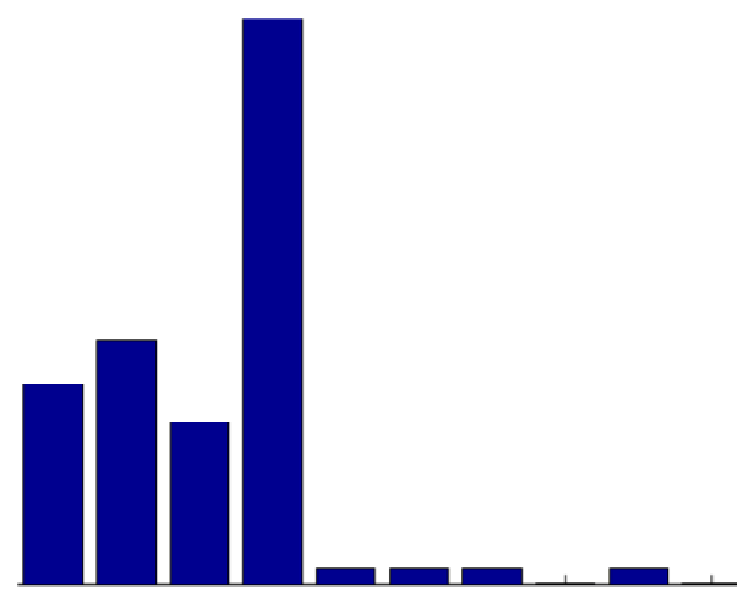
\includegraphics[width=0.24\textwidth, height=8mm]{s2} &
\includegraphics[width=0.24\textwidth, height=8mm]{s3}  \\
\vspace{-10mm}\hspace{0mm}\scalebox{0.72}{
\rotatebox[origin=r]{90}{reaching}\hspace{0.9mm}
\rotatebox[origin=r]{90}{moving}\hspace{0.9mm}
\rotatebox[origin=r]{90}{pouring}\hspace{0.9mm}
\rotatebox[origin=r]{90}{eating}\hspace{0.9mm}
\rotatebox[origin=r]{90}{drinking}\hspace{0.9mm}
\rotatebox[origin=r]{90}{opening}\hspace{0.9mm}
\rotatebox[origin=r]{90}{placing}\hspace{0.9mm}
\rotatebox[origin=r]{90}{closing}\hspace{0.9mm}
\rotatebox[origin=r]{90}{null}\hspace{0.9mm}
\rotatebox[origin=r]{90}{cleaning}}&
\vspace{-10mm}\hspace{-0.9mm}\scalebox{0.72}{
\rotatebox[origin=r]{90}{reaching}\hspace{0.9mm}
\rotatebox[origin=r]{90}{moving}\hspace{0.9mm}
\rotatebox[origin=r]{90}{pouring}\hspace{0.9mm}
\rotatebox[origin=r]{90}{eating}\hspace{0.9mm}
\rotatebox[origin=r]{90}{drinking}\hspace{0.9mm}
\rotatebox[origin=r]{90}{opening}\hspace{0.9mm}
\rotatebox[origin=r]{90}{placing}\hspace{0.9mm}
\rotatebox[origin=r]{90}{closing}\hspace{0.9mm}
\rotatebox[origin=r]{90}{null}\hspace{0.9mm}
\rotatebox[origin=r]{90}{cleaning}}&
\vspace{-10mm}\hspace{-0.9mm}\scalebox{0.72}{
\rotatebox[origin=r]{90}{reaching}\hspace{0.9mm}
\rotatebox[origin=r]{90}{moving}\hspace{0.9mm}
\rotatebox[origin=r]{90}{pouring}\hspace{0.9mm}
\rotatebox[origin=r]{90}{eating}\hspace{0.9mm}
\rotatebox[origin=r]{90}{drinking}\hspace{0.9mm}
\rotatebox[origin=r]{90}{opening}\hspace{0.9mm}
\rotatebox[origin=r]{90}{placing}\hspace{0.9mm}
\rotatebox[origin=r]{90}{closing}\hspace{0.9mm}
\rotatebox[origin=r]{90}{null}\hspace{0.9mm}
\rotatebox[origin=r]{90}{cleaning}}&
\vspace{-10mm}\hspace{-0.9mm}\scalebox{0.72}{
\rotatebox[origin=r]{90}{reaching}\hspace{0.9mm}
\rotatebox[origin=r]{90}{moving}\hspace{0.9mm}
\rotatebox[origin=r]{90}{pouring}\hspace{0.9mm}
\rotatebox[origin=r]{90}{eating}\hspace{0.9mm}
\rotatebox[origin=r]{90}{drinking}\hspace{0.9mm}
\rotatebox[origin=r]{90}{opening}\hspace{0.9mm}
\rotatebox[origin=r]{90}{placing}\hspace{0.9mm}
\rotatebox[origin=r]{90}{closing}\hspace{0.9mm}
\rotatebox[origin=r]{90}{null}\hspace{0.9mm}
\rotatebox[origin=r]{90}{cleaning}}
\end{tabular}
\end{tabular}

\vspace{7mm}


\begin{tabular}{p{3mm}@{}l}
\begin{tabular}{l}
\rotatebox[origin=r]{90}{\;\;\;\;\;\;Middle Frame}\\
\rotatebox[origin=l]{90}{Belief\;\;}
\end{tabular}
&
\begin{tabular}{p{3.2cm}p{3.2cm}p{3.2cm}p{3.2cm}}
\includegraphics[width=0.24\textwidth]{eat1} &
\includegraphics[width=0.24\textwidth]{eat2} &
\includegraphics[width=0.24\textwidth]{eat3} &
\includegraphics[width=0.24\textwidth]{eat4}  \\ %\\%\begin{tabular}{p{3.6cm}p{3.6cm}p{3.6cm}p{3.6cm}}
\includegraphics[width=0.24\textwidth, height=8mm]{et1} &
\includegraphics[width=0.24\textwidth, height=8mm]{et2} &
\includegraphics[width=0.24\textwidth, height=8mm]{et3} &
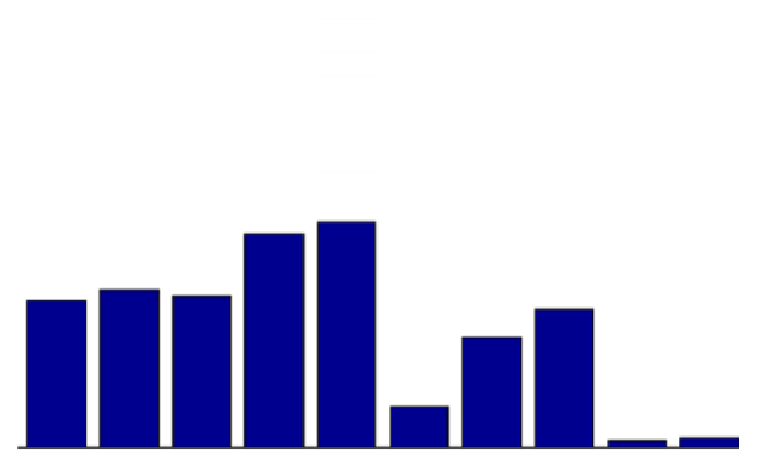
\includegraphics[width=0.24\textwidth, height=8mm]{et4}  \\
\vspace{-10mm}\hspace{0mm}\scalebox{0.72}{
\rotatebox[origin=r]{90}{reaching}\hspace{0.9mm}
\rotatebox[origin=r]{90}{moving}\hspace{0.9mm}
\rotatebox[origin=r]{90}{pouring}\hspace{0.9mm}
\rotatebox[origin=r]{90}{eating}\hspace{0.9mm}
\rotatebox[origin=r]{90}{drinking}\hspace{0.9mm}
\rotatebox[origin=r]{90}{opening}\hspace{0.9mm}
\rotatebox[origin=r]{90}{placing}\hspace{0.9mm}
\rotatebox[origin=r]{90}{closing}\hspace{0.9mm}
\rotatebox[origin=r]{90}{null}\hspace{0.9mm}
\rotatebox[origin=r]{90}{cleaning}}&
\vspace{-10mm}\hspace{-0.9mm}\scalebox{0.72}{
\rotatebox[origin=r]{90}{reaching}\hspace{0.9mm}
\rotatebox[origin=r]{90}{moving}\hspace{0.9mm}
\rotatebox[origin=r]{90}{pouring}\hspace{0.9mm}
\rotatebox[origin=r]{90}{eating}\hspace{0.9mm}
\rotatebox[origin=r]{90}{drinking}\hspace{0.9mm}
\rotatebox[origin=r]{90}{opening}\hspace{0.9mm}
\rotatebox[origin=r]{90}{placing}\hspace{0.9mm}
\rotatebox[origin=r]{90}{closing}\hspace{0.9mm}
\rotatebox[origin=r]{90}{null}\hspace{0.9mm}
\rotatebox[origin=r]{90}{cleaning}}&
\vspace{-10mm}\hspace{-0.9mm}\scalebox{0.72}{
\rotatebox[origin=r]{90}{reaching}\hspace{0.9mm}
\rotatebox[origin=r]{90}{moving}\hspace{0.9mm}
\rotatebox[origin=r]{90}{pouring}\hspace{0.9mm}
\rotatebox[origin=r]{90}{eating}\hspace{0.9mm}
\rotatebox[origin=r]{90}{drinking}\hspace{0.9mm}
\rotatebox[origin=r]{90}{opening}\hspace{0.9mm}
\rotatebox[origin=r]{90}{placing}\hspace{0.9mm}
\rotatebox[origin=r]{90}{closing}\hspace{0.9mm}
\rotatebox[origin=r]{90}{null}\hspace{0.9mm}
\rotatebox[origin=r]{90}{cleaning}}&
\vspace{-10mm}\hspace{-0.9mm}\scalebox{0.72}{
\rotatebox[origin=r]{90}{reaching}\hspace{0.9mm}
\rotatebox[origin=r]{90}{moving}\hspace{0.9mm}
\rotatebox[origin=r]{90}{pouring}\hspace{0.9mm}
\rotatebox[origin=r]{90}{eating}\hspace{0.9mm}
\rotatebox[origin=r]{90}{drinking}\hspace{0.9mm}
\rotatebox[origin=r]{90}{opening}\hspace{0.9mm}
\rotatebox[origin=r]{90}{placing}\hspace{0.9mm}
\rotatebox[origin=r]{90}{closing}\hspace{0.9mm}
\rotatebox[origin=r]{90}{null}\hspace{0.9mm}
\rotatebox[origin=r]{90}{cleaning}}
\end{tabular}
\end{tabular}

\vspace{7mm}

\begin{tabular}{p{3mm}@{}l}
\begin{tabular}{l}
\rotatebox[origin=r]{90}{\;\;\;\;\;\;Middle Frame}\\
\rotatebox[origin=l]{90}{Belief\;\;}
\end{tabular}
&
\begin{tabular}{p{3.2cm}p{3.2cm}p{3.2cm}p{3.2cm}}
\includegraphics[width=0.24\textwidth]{ff2} &
\includegraphics[width=0.24\textwidth]{ff3} &
\includegraphics[width=0.24\textwidth]{ff4} &
\includegraphics[width=0.24\textwidth]{ff5}  \\ %\\%\begin{tabular}{p{3.6cm}p{3.6cm}p{3.6cm}p{3.6cm}}
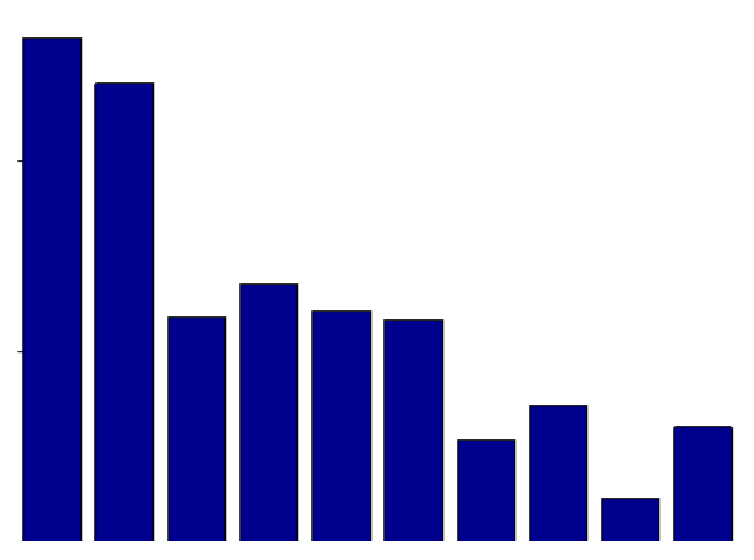
\includegraphics[width=0.24\textwidth, height=8mm]{b2} &
\includegraphics[width=0.24\textwidth, height=8mm]{bb3} &
\includegraphics[width=0.24\textwidth, height=8mm]{bb4} &
\includegraphics[width=0.24\textwidth, height=8mm]{bb5}  \\
\vspace{-10mm}\hspace{0mm}\scalebox{0.72}{
\rotatebox[origin=r]{90}{reaching}\hspace{0.9mm}
\rotatebox[origin=r]{90}{moving}\hspace{0.9mm}
\rotatebox[origin=r]{90}{pouring}\hspace{0.9mm}
\rotatebox[origin=r]{90}{eating}\hspace{0.9mm}
\rotatebox[origin=r]{90}{drinking}\hspace{0.9mm}
\rotatebox[origin=r]{90}{opening}\hspace{0.9mm}
\rotatebox[origin=r]{90}{placing}\hspace{0.9mm}
\rotatebox[origin=r]{90}{closing}\hspace{0.9mm}
\rotatebox[origin=r]{90}{null}\hspace{0.9mm}
\rotatebox[origin=r]{90}{cleaning}}&
\vspace{-10mm}\hspace{-0.9mm}\scalebox{0.72}{
\rotatebox[origin=r]{90}{reaching}\hspace{0.9mm}
\rotatebox[origin=r]{90}{moving}\hspace{0.9mm}
\rotatebox[origin=r]{90}{pouring}\hspace{0.9mm}
\rotatebox[origin=r]{90}{eating}\hspace{0.9mm}
\rotatebox[origin=r]{90}{drinking}\hspace{0.9mm}
\rotatebox[origin=r]{90}{opening}\hspace{0.9mm}
\rotatebox[origin=r]{90}{placing}\hspace{0.9mm}
\rotatebox[origin=r]{90}{closing}\hspace{0.9mm}
\rotatebox[origin=r]{90}{null}\hspace{0.9mm}
\rotatebox[origin=r]{90}{cleaning}}&
\vspace{-10mm}\hspace{-0.9mm}\scalebox{0.72}{
\rotatebox[origin=r]{90}{reaching}\hspace{0.9mm}
\rotatebox[origin=r]{90}{moving}\hspace{0.9mm}
\rotatebox[origin=r]{90}{pouring}\hspace{0.9mm}
\rotatebox[origin=r]{90}{eating}\hspace{0.9mm}
\rotatebox[origin=r]{90}{drinking}\hspace{0.9mm}
\rotatebox[origin=r]{90}{opening}\hspace{0.9mm}
\rotatebox[origin=r]{90}{placing}\hspace{0.9mm}
\rotatebox[origin=r]{90}{closing}\hspace{0.9mm}
\rotatebox[origin=r]{90}{null}\hspace{0.9mm}
\rotatebox[origin=r]{90}{cleaning}}&
\vspace{-10mm}\hspace{-0.9mm}\scalebox{0.72}{
\rotatebox[origin=r]{90}{reaching}\hspace{0.9mm}
\rotatebox[origin=r]{90}{moving}\hspace{0.9mm}
\rotatebox[origin=r]{90}{pouring}\hspace{0.9mm}
\rotatebox[origin=r]{90}{eating}\hspace{0.9mm}
\rotatebox[origin=r]{90}{drinking}\hspace{0.9mm}
\rotatebox[origin=r]{90}{opening}\hspace{0.9mm}
\rotatebox[origin=r]{90}{placing}\hspace{0.9mm}
\rotatebox[origin=r]{90}{closing}\hspace{0.9mm}
\rotatebox[origin=r]{90}{null}\hspace{0.9mm}
\rotatebox[origin=r]{90}{cleaning}}
\end{tabular}
\end{tabular}
\normalsize
\caption{\textbf{Anticipated belief over activity.} In the odd numbered rows, we show a middle frame of the temporal segment. In the even numbered rows, we show the anticipated belief. Note that frames are not visible to the algorithm and only included for evaluation.}
\label{abcd}
\end{figure}



\section{Quantitative Results}
\begin{table}[ht]
\centering
\tabcolsep=0.7mm
\footnotesize
%\vspace{-1mm}
\caption{\textbf{Anticipation performance for the anticipating 3 seconds in the future.} We compare rCRF with state-of-the-art anticipation algorithm and baselines for anticipation accuracy. rCRF outperforms the state-of-the-art heuristic method \cite{hemaAnt} and the GP-LCRF method \cite{gpcrf} significantly as well as all other baselines. We believe this result is due to the accurate joint-modeling of the temporal relations and the CRF model.}
\vspace{-1mm}
\resizebox{1\columnwidth}{!}{
\begin{tabular}{@{}l@{}|ccc|ccc@{}} \hline
& \multicolumn{3}{@{}|c@{}}{Sub-activity } &   \multicolumn{3}{@{}|c@{}}{Object Affordance } \\ \hline
& micro & macro & robot ant. &  micro & macro & robot ant.   \\
Method & prec(\%) & f1-scr(\%) & metric(\%) & prec(\%) & f1-scr(\%) & metric(\%) \\ \hline
Chance & $10.0${\scriptsize $\pm 0.1$} & $10.0${\scriptsize $\pm 0.1$}  & $30.0${\scriptsize $\pm 0.1$} & $8.3${\scriptsize $\pm 0.1$} & $8.3${\scriptsize $\pm 0.1$}  & $24.9${\scriptsize $\pm 0.1$}  \\
GP-LCRF \cite{gpcrf} & $52.1${\scriptsize $\pm 1.2$} & $43.2${\scriptsize $\pm 1.5$} &  $76.1${\scriptsize $\pm 1.5$}  & $68.1${\scriptsize$\pm 1.0$}  & $44.2${\scriptsize $\pm 1.2$}  & $74.9${\scriptsize $\pm 1.1$}  \\
ATCRF \cite{hemaAnt} & $47.7${\scriptsize $\pm 1.6$} & $37.9${\scriptsize $\pm 2.6$} &  $69.2${\scriptsize $\pm 2.1$}  & $66.1${\scriptsize $\pm 1.9$}  & $36.7 ${\scriptsize $\pm 2.3$}  & $71.3${\scriptsize $\pm 1.7$}  \\
DivMBest\cite{divmbest}& $47.9${\scriptsize $\pm 1.4$} & $43.2${\scriptsize $\pm 3.6$} & $71.5${\scriptsize $\pm 2.7$} & $61.3${\scriptsize $\pm 1.4$} & $56.3 ${\scriptsize $\pm 2.1$} & $73.3${\scriptsize $\pm 0.5$} \\
DCRF\cite{ddcrf}& $48.3${\scriptsize $\pm 2.6$} & $35.4${\scriptsize $\pm 1.8$} & $66.6${\scriptsize $\pm 1.1$} &
$55.2${\scriptsize $\pm 3.1$} & $48.5${\scriptsize $\pm 3.1$} & $71.24${\scriptsize $\pm 2.2$} \\
rCRF w/o div& $49.6${\scriptsize $\pm 2.1$} & $39.7${\scriptsize $\pm 2.6$} & $65.1${\scriptsize $\pm 1.1$} & $56.2${\scriptsize $\pm 1.9$} & $47.4${\scriptsize $\pm 3.1$} & $70.8${\scriptsize $\pm 2.5$} \\
rCRF & $\mathbf{54.3}${\scriptsize $\mathbf{\pm 3.9}$} & $\mathbf{45.8}${\scriptsize $\mathbf{\pm 2.7}$} & $\mathbf{76.5}${\scriptsize $\mathbf{\pm 2.6 }$}  & $\mathbf{78.7}${\scriptsize $\mathbf{\pm 3.4}$} &$\mathbf{74.9}${\scriptsize $\mathbf{\pm 3.8}$} & $\mathbf{82.1}${\scriptsize $\mathbf{\pm 2.9}$} \\
\hline
\end{tabular}}
\label{Tant}
\end{table}

\begin{figure}[t]
  \centering
  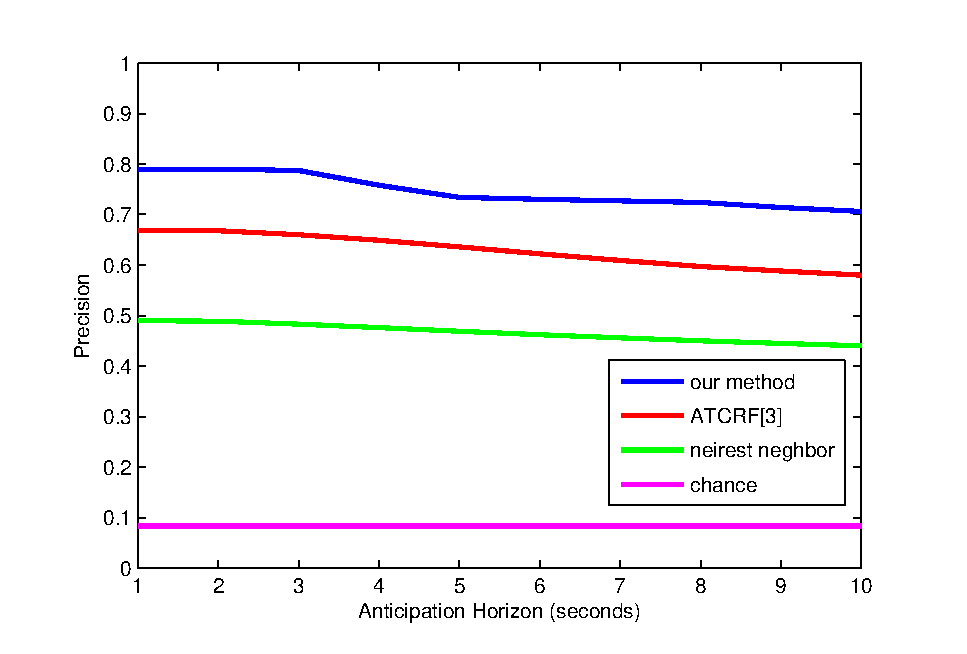
\includegraphics[width=0.48 \textwidth]{AntO}
\caption{Precision vs. anticipation horizon for object affordance. We run all possible experiments for $\tau$ seconds into the future experiments as showing $t$ seconds of the video and anticipating $t+\tau$ for all $t<T-\tau$}
\label{antHor}
\end{figure}




\noindent {\bf Computationally-efficient inference:}
We evaluated the computational efficiency by computing the average computation time for anticipating 3 second in the future via rCRF and the fastest available anticipation algorithm (the ATCRF\cite{hemaAnt}). Within our experiments, we did not include any pre-processing or feature extraction computation (they are same for all algorithms).
\begin{table}[h!]
  \centering
%  \vspace{-2mm}
\caption{Computation time for anticipating 3 seconds in the future excluding pre-processing (\emph{see supplementary material for details}).}
%\vspace{-2mm}
  \begin{tabular}{|cc|cc|}
    \hline
  ATCRF \cite{hemaAnt} \; \; & \; \; 34.1s  \; \;  \; & \; \; \;  rCRF \; \; & \; \;  1.41s \\ \hline
  \end{tabular}
  \vspace{-1mm}
  \label{speed}
\end{table}
%\vspace{-2mm}


\end{document}
